\documentclass[a4paper, 12pt]{book}

\usepackage[T1]{fontenc}
\usepackage[utf8]{inputenc}
\usepackage[italian]{babel}
\usepackage{quoting}
\usepackage{graphicx} %per inserire immagini nel testo
\usepackage{sidecap} %permette di aggiungere didascalie alle immagini
\usepackage{subfig}
\usepackage[colorlinks]{hyperref} %per rendere interattivo il documento, gli elementi interattivi saranno in rosso con l'opzione colorlinks
\usepackage{amsmath}
\usepackage{amsthm} %per enunciati
\theoremstyle{plain}
\newtheorem{teorema}{Teorema}[section]
\usepackage{geometry}
\geometry{a4paper, top = 3cm, bottom = 3cm, left = 3.5cm, right = 3.5cm, heightrounded, bindingoffset = 5mm}
\pagestyle{plain}
\usepackage{multirow}
\setcounter{secnumdepth}{3}

\title{Sistemi}
\author{Giovanni Tosini}
\date{ }

\begin{document}

\begin{titlepage}
    \maketitle
\end{titlepage}

\frontmatter
\tableofcontents
\mainmatter

\chapter{Numeri complessi}

Un numero complesso $s = \sigma + j\omega$ con $j = \sqrt{-1}$ e $\sigma , \omega \in R$ in cui 
\begin{itemize}
    \item $\sigma = Re(s)$ parte reale
    \item $\omega = Im(s)$ parte immaginaria
    \item $C = {s t.c. s = \sigma + j\omega, \sigma , \omega \in R}$ insieme dei numeri complessi
\end{itemize}
\begin{center}
    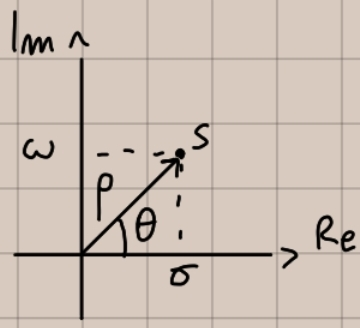
\includegraphics[width=0.5\textwidth]{num_comp.jpg}
\end{center}
Forma polare dei numeri complessi, $s = \rho (cos\theta +jsin\theta)$
\begin{itemize}
    \item $\rho = \sqrt{\sigma ^2+\omega ^2}$ il modulo di $s$ con $\rho \in R^+$
    \item $\theta =$ argomento di $s$
\end{itemize}
\begin{description}
    \item[Osservazione 1] $Re(s) = \rho cos\theta$ e $Im(s) = \rho sin\theta$
    \item[Osservazione 2] L'argomento $\theta$ è determinato a meno di multipli interi di 
            $2\pi$. Imponendo $\theta \in [0, 2\pi )$ oppure $(-\pi , \pi ]$ (deve essere un intervallo
            lungo $2\pi$ ) si ottiene l'argomento principale $\theta$ che notiamo con $arg(s)$  
\end{description}

\section{Formula di Eulero}

$\theta \in R, j = \sqrt{-1}$ abbiamo $e^{j\theta}=cos\theta +jsin\theta$

\paragraph{Forma esponenziale}

$s=\rho e^{j\theta}$
\begin{center}
    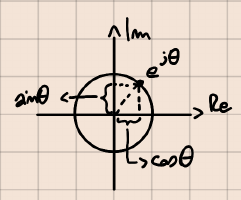
\includegraphics[width=0.5\textwidth]{num_comp2.png}
\end{center}
$|e^{j\theta}=\sqrt{cos^2\theta +sin^2\theta} = 1$

Esempio: $e^{j\frac{\pi}{2}}=j$
\begin{center}
    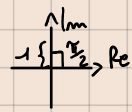
\includegraphics[width=0.5\textwidth]{num_comp3.png}
\end{center}
$s=0+1j=j$
\begin{description}
    \item[Def:] i numeri \textbf{immaginari puri} hanno la parte reale nulla
    \item[Def:] dato $s: \sigma + j\omega \in C$ $\bar{s}: \sigma - j\omega$ coniugato complesso   
\end{description}
\begin{center}
    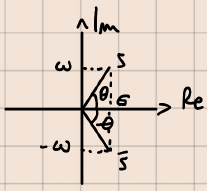
\includegraphics[width=0.5\textwidth]{num_comp4.png}
\end{center}
La forma polare di $\bar{s}$ sarà uguale a $\rho (cos\theta - jsin\theta)$
\begin{description}
    \item[Osservazione] $|s|=|\bar{s}| arg(\bar{s})=-arg(s)$ 
\end{description}

Esempio: $e^{j\pi}=-1=e^{j\pi}+1=0$
\begin{center}
    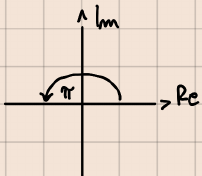
\includegraphics[width=0.5\textwidth]{num_comp5.png}
\end{center}

\section{Operazioni con i numero complessi}

\begin{itemize}
    \item $s_1=\sigma_1+j\omega_1,s_2=\sigma_2+j\omega_2\in C$
    \item $s_1+s_2=\sigma_1+\sigma_2+j(\omega_1+\omega_2)$
    \item $s_1-s_2=\sigma_1-\sigma_2+j(\omega_1-\omega_2)$
\end{itemize}
\begin{description}
    \item[Osservazione:] $Re(s)=\frac{s+\bar{s}}{2}$ e $Im(s)=\frac{s+\bar{s}}{2j}$ 
\end{description}
Per la formula di Eulero $e^{j\theta}=cos\theta+jsin\theta \Rightarrow cos\theta = \frac{e^{j\theta}+e^{-j\theta}}{2}$ e
$sin\theta =\frac{e^{j\theta} -e^{-j\theta}}{2j}$
\begin{center}
    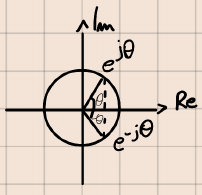
\includegraphics[width=0.5\textwidth]{num_comp6.png}
\end{center}
\begin{description}
    \item[Osservazione:]$2Re(s)=s+\bar{s}$ e $2jIm(s)=s-\bar{s}$ 
\end{description}
$s=\bar{s} \Rightarrow Im(s)=0$ e $s=-\bar{s} \Rightarrow Re(s)=0$
\begin{center}
    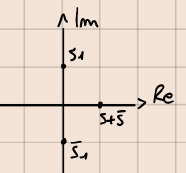
\includegraphics[width=0.5\textwidth]{num_comp7.png}
    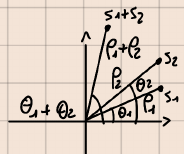
\includegraphics[width=0.5\textwidth]{num_comp8.png}
\end{center}
\begin{itemize}
    \item $s_1 = \rho_1(cos\theta_1+jsin\theta_1)$
    \item $s_2 = \rho_1(cos\theta_2+jsin\theta_2)$
    \item $s_1s_2=\rho_1\rho_2(cos(\theta_1+\theta_2)+jsin(\theta_1+\theta_2))$
    \item $s_1s_2=\rho_1\rho_2(cos\theta_1cos\theta_2+jcos\theta_1sin\theta_2+jsin\theta_1cos\theta_2-sin\theta_1sin\theta_2)$
    \item $s_1s_2=\rho_1\rho_2(cos\theta_1cos\theta_2-sin\theta_1sin\theta_2+j(cos\theta_1sin\theta_2+sin\theta_1cos\theta_2))$
\end{itemize}
\begin{description}
    \item[N.B.:] $cos\theta_1cos\theta_2-sin\theta_1sin\theta_2=cos(\theta_1+\theta_2)$ e 
    $cos\theta_1sin\theta_2+sin\theta_1cos\theta_2=sin(\theta_1+\theta_2)$
    \item [Def:]Dato $s\in C$ il numero $s^{-1}$ t.c. $ss^{-1}=1$, $s^{-1}=\frac{\bar{s}}{|s|^2}$ reciproco
    (inverso) di $s$.
    \item $ss^{-1}=s\frac{\bar{s}}{|s|^2}=\frac{s\bar{s}}{|s|^2}$
    \item $s\bar{s}=\rho^2(cos(\theta-\theta)+jsin(\theta-\theta))=\rho^2=|s|^2$
    \item [Osservazione:]l'argomento di un numero complesso si può chiamare anche \textbf{fase}.
    \item $\frac{s_1}{s_2}=s_1s_2^{-1}=s_1\frac{\bar{s_2}}{|s_2|^2}=\frac{\rho_1}{\rho_2}(cos(\theta_1-\theta_2)
    jsin(\theta_1-\theta_2))$
    \item [Osservazione:] $s\bar{s}=\rho^2(cos(\theta-\theta)+jsin(\theta-\theta))=\rho^2\Rightarrow|s|^2=s\bar{s}$ 
\end{description}
\begin{center}
    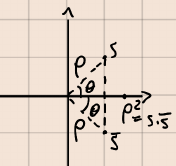
\includegraphics[width=0.5\textwidth]{num_comp9.png}
\end{center}
\begin{description}
    \item[Def: ]$u\in C$ si dice complesso unitario se $|u|=1$. In forma polare $u=cos\theta+jsin\theta$. In forma esponenziale
     $u=e^{j\theta}$ e $|e^{j\theta}|=1$  
\end{description}
Sia $u=cos\alpha+jsin\alpha$ con $s=\rho(cos\theta+jsin\theta)$ avremo che $su=\rho(cos(\theta+\alpha)+jsin(\theta+\alpha))$
(rotazione intorno all'origine)
\begin{center}
    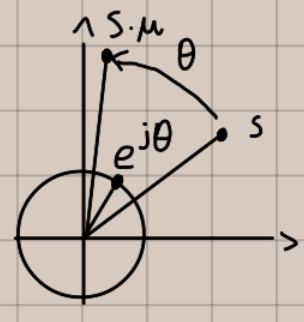
\includegraphics[width=0.5\textwidth]{num_comp10.jpg}
\end{center}
$s^n=\rho^n(cos(n\theta)+jsin(n\theta))$

Esempio: \[(e^{j\theta})^n=e^{jn\theta}\]
\paragraph{Radici complesse}

Ogni $s\in C$ ammette $n$ distinte radici $n$-esime $\omega_1,\dots,\omega_{n-1} \in C$.
Dobbiamo trovare $\omega \in C$ t.c. $\omega^n=s$.
\[]\forall k \in [0, n-1], \omega_k\sqrt[n]{\rho}(cos(\frac{\theta}{n}+\frac{2\pi}{n}k)
+jsin(\frac{\theta}{n}+\frac{2\pi}{n}k))
\]
Prova: 
\[
\begin{split}
\omega_k^n &= (\sqrt[n]{\rho}^n)(\cos(n(\frac{\theta}{n}+\frac{2\pi}{n}k))+jsin(n(\frac{\theta}{n}+\frac{2\pi}{n}k))) = \\
 &= \rho(cos(\theta+2\pi k)+jsin(\theta+2\pi k))= \\
\end{split}
\]
Notare che $cos(\theta+2\pi k)$ è equivalente a $cos\theta$ e $sin(\theta+2\pi k)$ equivale a $sin\theta$ questo
$\forall k=0,...,n-1$.

L'equazione: $s^4=1+2j$ ha 4 radici distinte nel campo $C$.
Esempio: le radici complesse dell'unità

$s^n=1 \omega_k=cos(\frac{2\pi}{n}k) + jsin(\frac{2\pi}{n}k) k=0,...,n-1$

\paragraph{Funzioni di variabile complessa}

Gli insieme su cui definiamo una funzione di variabile complessa
 f si scrivono $D(f)$, $D(f)\subseteq C$
 \begin{description}
     \item[Def: ]un punto $s_0\in D(f)\subseteq C$ è interno a $D(f)$
     se esiste un disco $B_\rho(s_0)$ di raggio $\rho$ con $\rho\in R^+$ centrato
     in $s_0$, t.c. $B_\rho(s_0)\subseteq D(f)$ dove $B_\rho(s_0)={s\in C t.c. |s-s_0| < \rho}$
 \end{description}
 \begin{center}
     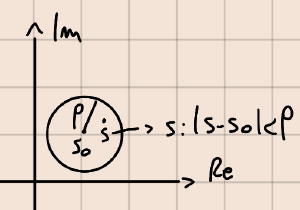
\includegraphics[width=0.5\textwidth]{num_comp11.png}
 \end{center}
 \begin{description}
     \item[Def: ]Un insieme $D(f)\subseteq C$ si dice aperto se tutti i suoi punti
     sono interni 
     \item [Def: ]Una funzione $f:D(f)\rightarrow C$ con $D(f)\subseteq C$ aperto
     è una funzione complessa
 \end{description}
 Esempi di funzioni complesse con annesso dominio:
 \begin{itemize}
     \item $f(s) = s, D(f) = C$
     \item $f(s)=s^2,D(f)=C$
     \item $f(s)=Re(s)+jIm(s)^2, D(f)=C$
     \item $f(s)=\sum_{k=0}^n a_ks^k, D(f)=C$
     \item funzione polinomiale, $f(s)=\frac{P(s)}{Q(s)}$ dove $P(s)=\sum_{k=0}^n a_ks^k$ e funzione razionale $Q(s)=\sum_{k=0}^n b_ks^k$,
     $D=C-{\lambda_1,...,\lambda_m}$ dove $\lambda_\alpha$ è radice di $Q(s)=0$ per $k=1,...,m$
 \end{itemize}
 \section{Teorema fondamentale dell'algebra}
 Ogni polinomio $P(s)$ a coefficienti complessi di grado $n>0$ ha $n$ radici complesse e si può comporre come
 \begin{center}
         $P(s) = a_n(s-\lambda_1)^\mu_1(s-\lambda_2)^\mu_2...(s-\lambda_r)^\mu_r$ dove 
        $\lambda_1,...\lambda_r$ sono radici  e $\mu_1,...,\mu_r$ sono le \textbf{molteplicità} relative di ciascuna
        radice per cui $\mu_1 + ... + \mu_r = n$
 \end{center}
 \begin{description}
     \item[Osservazione] Un numero $\lambda$ è una radice di molteplicità $\mu$ per un polinomio $P(s)$
    se e solo se $P(\lambda)=P'(\lambda)=P''(\lambda)=...=P^{\mu - 1}(\lambda) = 0$ e $P^\mu (\lambda)\neq 0$
    \end{description}

\chapter{Segnali}

Sono funzioni matematiche definite su un dominio, esistono nel dominio:
\begin{itemize}
    \item continuo $\rightarrow R, C, \dots$;
    \item discreto $\rightarrow Z$.
\end{itemize}

\section{Segnali elementari a tempo continuo}
\subsection{Segnale sinusoidale}
Consiste di una funzione:
\[
v: R \rightarrow R, v(t) = A \overbrace{\cos}^{[-1, 1]}(\omega t + \phi)
\textrm{ con } A, \omega, \phi \in R 
\]
\begin{itemize}
    \item $A > 0$ è l'ampiezza;
    \item $\omega$ la pulsazione;
    \item $\phi$ la fase;
    \item $v$ è periodico di periodo $T = \frac{2\pi}{\omega}$;
    \item la frequenza $f = \frac{1}{T} \rightarrow f = \frac{\omega}{2\pi}$.
\end{itemize}

\begin{SCfigure}[50][h!]
    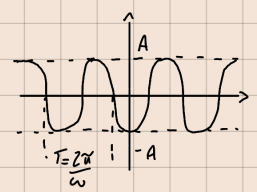
\includegraphics[width=0.5\textwidth]{sinusoidale.png}
    \caption{Funzione sinusoidale}
\end{SCfigure}

\subsection{Fasore}
Una funzione:
\[
v : R \rightarrow C, v(t) = A e^{j(\omega t + \phi)}\footnote{$e^{j\theta} = \cos \theta + j\sin \theta \rightarrow
|e^{j\theta}| = 1$} 
\textrm{ con } A, \omega, \phi \in R    
\]
Di conseguenza sarà uguale sempre ad $A$.
\begin{description}
    \item[Osservazione: ] dalla formulla di Eulero, possiamo esprimere
    un segnale sinusoidale \[\begin{split}
        A \cos (\omega t + \phi) &= A\frac{e^{j(\omega t + \phi)} + e^{-j(\omega t + \phi)}}{2} = \\
        &= \frac{A}{2} e^{j(\omega t + \phi)} + \frac{A}{2} e^{-j(\omega t + \phi)} \\
    \end{split} \]  
\end{description}

\begin{SCfigure}[50][h!]
    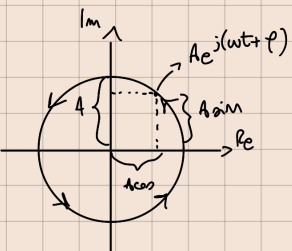
\includegraphics[width=0.5\textwidth]{fasore.png}
    \caption{Fasore}
\end{SCfigure}

\subsection{Segnale sinusoidale modulato esponenzialmente}

\begin{gather}
    v : R \rightarrow R\\
    v(t) = A e^{\sigma t} \cos (\omega t + \phi)\\
    \textrm{ con } \sigma, A, \omega, \phi \in R, A > 0\\
\end{gather}
 \textbf{non} è periodico.   

\begin{itemize}
    \item per $\sigma > 0$ e $t \rightarrow \infty \Rightarrow v(t) = \infty$
    \item per $\sigma < 0$ e $t \rightarrow \infty \Rightarrow v(t) = 0$
\end{itemize}

\begin{SCfigure}[50][h!]
    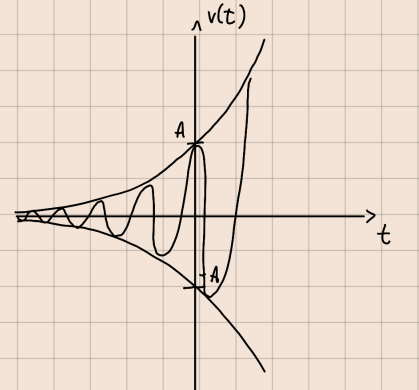
\includegraphics[width=0.3\textwidth]{nomelunghissimo.png}
    \caption{Segnale sinusoidale modulato esponenzialmente}
\end{SCfigure}

\begin{description}
    \item[Osservazione: ] segnali sinusoidali, modulati esponenzialmente, si possono scrivere come combinazione lineare di fasori con una componente esponenziale: \[
        \begin{split}
            A e^{\sigma t} \cos (\omega t + \phi) &= A e^{\sigma t} \frac{e^{j(\omega t + \phi)} + e^{-j(\omega t + \phi)}}{2} = \\
            &= \frac{A e^{\sigma t} e^{j(\omega t + \phi)}}{2} + \frac{A e^{\sigma t} e^{-j(\omega t - \phi)}}{2} = \\
            &= \underbrace{\frac{A}{2} e^{\sigma t} e^{j\omega t + j\phi} + \frac{A}{2} e^{\sigma t} e^{-j\omega t - j\phi}}_{\textrm{sono complessi coniugati}}
        \end{split}
         \] 
\end{description}

\subsection{Segnale esponenziale complesso}
\[
v : R \rightarrow C, v(t) = A e^{\sigma t} e^{j(\omega t + \phi)}
\]

\begin{figure}[h!]
    \centering
		\subfloat[][\textbf{\emph{Per $\sigma > 0$ e $t \rightarrow \infty |v(t)| \rightarrow \infty$}}]
		{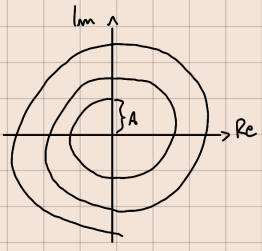
\includegraphics[width=0.3\textwidth]{uzumaki1.png}}\quad
		\subfloat[][\textbf{\emph{Per $\sigma < 0$ e $t \rightarrow \infty |v(t)| \rightarrow 0$}}]
		{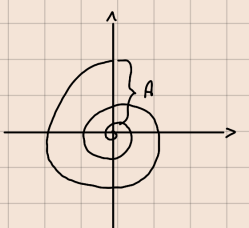
\includegraphics[width=0.3\textwidth]{uzumaki2.png}}\\
\end{figure}

\subsection{Funzioni generalizzate}
\subsubsection{Segnali polinomiali}
\[
\delta_{-n} : R \rightarrow R \\
\delta_{-n} = \begin{cases}
    \frac{t^{n - 1}}{(n - 1)!}, t \ge 0;\\
    0 \textrm{, altrimenti}
\end{cases}    
\]

Da un certo istante ha un valore e quello sarà l'istante 0.
\begin{description}
    \item[Osservazione: ] \[
    \delta_{-n}(t) = \int_{-\infty}^t \delta_{-(n - 1)}(\Psi)d\Psi    
    \] 
    Il segnale polinomiale n-esimo può essere ottenuto come integrale del segnale (n - 1)-esimo
    \[
    \delta_{-n}(t) = \frac{d\delta_{-(n + 1)}^t}{dt}\]
\end{description}
Esempio per n = $1$
\[\delta_{-1}(t) = 
\begin{cases}
    1, t \ge 0\\
    0, \textrm{altrimenti}
\end{cases}    
\]

Per n = $2$
\[\delta_{-2}(t) =
\begin{cases}
    t, t \ge 0\\
    0, \textrm{altrimenti}
\end{cases}
\]

\begin{figure}[h!]
    \centering
		\subfloat[][\textbf{\emph{Funzione gradino}}]
		{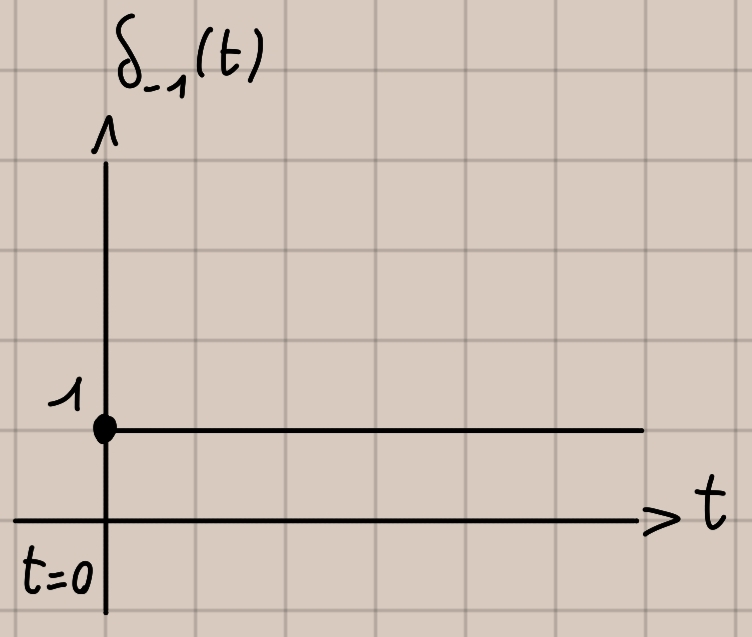
\includegraphics[width=0.3\textwidth]{gradino.jpg}}\quad
		\subfloat[][\textbf{\emph{Rampa unitaria}}]
		{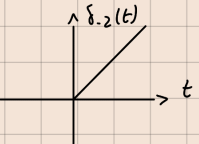
\includegraphics[width=0.3\textwidth]{rampa.png}}\\
\end{figure}

\begin{description}
    \item[Osservazione: ] l'integrale del gradino è la rampa e viceversa la derivata della rampa è il gradino.
\end{description}
\[
    \int_{-\infty}^{t}\delta_{-1}d\alpha = \delta_{-2}(t) \\
    \frac{d\delta_{-2}(t)}{dt} = \delta_{-1}(t)  
\]

\subsubsection{Finestra rettangolare unitaria}

\[
    \Pi : R \rightarrow R \Pi(t) = \begin{cases}
        1, -\frac{1}{2} \le t \le \frac{1}{2}\footnote{Il supporto = $(-\frac{1}{2}, \frac{1}{2}) \subset R$}\\
        0, \textrm{altrimenti}
    \end{cases}    
\]

\begin{SCfigure}[50][h!]
    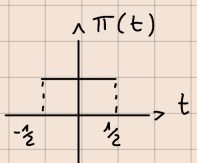
\includegraphics[width=0.3\textwidth]{finestra.png}
    \caption{Finestra rettangolare unitaria, ampiezza = $1$}
\end{SCfigure}

\begin{description}
    \item[Osservazione: ] La finestra rettangolare unitaria è una combinazione lineare di due gradini: 
\end{description}

\[
    \Pi(t) = \delta_{-1}(t + \frac{1}{2}) - \delta_{-1}(t - \frac{1}{2})
\]

\subsubsection{Finestra rettangolare ad ampiezza A con diverso supporto}

\begin{description}
    \item[N.B.:] il supporto è il sottoinsieme del dominio per cui la funzione è $\neq 0$
\end{description}

\begin{center}
    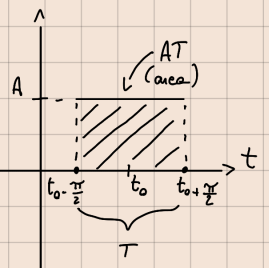
\includegraphics[width=0.3\textwidth]{finestra2.png}
\end{center}

L'ampiezza A, centrata in $t_0$, con supporto $(t_0 - \frac{\pi}{2}, t_0 + \frac{\pi}{2})$.
\[
    A\Pi(\frac{t - t_0}{T}) = \begin{cases}
        A, t_0 - \frac{\pi}{2} \le t \le t_0 + \frac{\pi}{2}\\
        0, \textrm{altrimenti}
    \end{cases}
\]

\subsubsection{Finestre (o impulso) triangolare unitaria}

\[
    \Lambda : R \rightarrow R, \Lambda(t) = \begin{cases}
        1 - |t|, -1 \le t \le 1\\
        0, \textrm{altrimenti}
    \end{cases}
\]

\begin{SCfigure}[50][h!]
    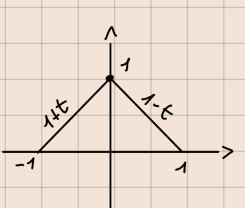
\includegraphics[width=0.3\textwidth]{triangolo.png}
    \caption{Impulso, supporto $[-1, 1]$, area = $1$}
\end{SCfigure}

\subsubsection{Finestra triangolare ad ampiezza A con supporto 2T centrata in $t_0$}

\begin{center}
    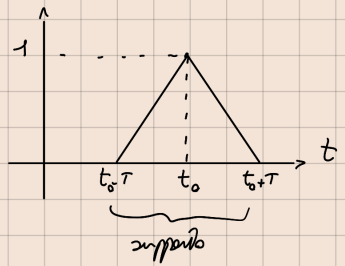
\includegraphics[width=0.5\textwidth]{triangolo2.png}
\end{center}

\[
    A\Lambda(\frac{t - t_0}{T}) = \begin{cases}
        A - \frac{A}{T} |t - t_0|, t_0 - T \le t \le t_0 + T\\
        0, \textrm{altrimenti}
    \end{cases}
\]
supporto $(t_0 - T, t_0 + T)$, area = $AT$

\subsubsection{Impulso di Dirac o funzione $\delta (t)$}
\begin{description}
    \item[Osservazione: ] l'impulso è una funzione generalizzata che è definita come un limite di una succesione di funzioni. 
\end{description}

\[
    \begin{split}
        \delta(t) &= \lim_{n \rightarrow \infty} \delta_n (t) =\\
        &= \lim_{n \rightarrow \infty} \frac{n}{2}\Pi(\frac{t}{\frac{2}{n}}) \textrm{ dove}\\
        f_n(t) &= \frac{n}{2}\Pi(\frac{t}{\frac{2}{n}}) = \\
        &=\begin{cases}
            \frac{n}{2}, -\frac{1}{n} \le t \le \frac{1}{n}\\
            0, \textrm{altrimenti}
        \end{cases}
    \end{split}  
\]

\begin{SCfigure}[50][h!]
    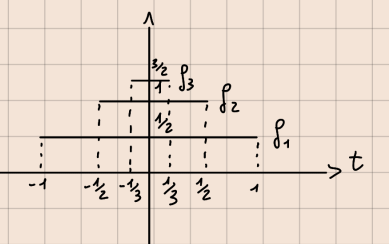
\includegraphics[width=0.5\textwidth]{dirac.png}
    \caption{Impulso di Dirac, prosegue fino a $\infty$}
\end{SCfigure}

\[
    \delta_t "=" \begin{cases}
        \infty, t = 0\\
        0, \textrm{altrimenti}
    \end{cases}
\]
\[
    \begin{split}
        \int_{-\infty}^\infty \delta(t) dt &= \int_{-\infty}^\infty \lim_{n \rightarrow \infty} f_n(t) dt = \\
        &= \lim_{n \rightarrow \infty} \int_{-\infty}^\infty \overbrace{f_n (t) dt}^{\textrm{ogni finestra ha area = 1}} = \\
        &= \lim_{n \rightarrow \infty} 1 = 1
    \end{split}
\]

\begin{SCfigure}[50][h!]
    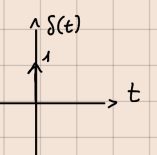
\includegraphics[width=0.5\textwidth]{frecciasu.png}
    \caption{Rappresentazione grafica}
\end{SCfigure}

\subsubsection{Impulso di ampiezza A e centrato in $t_0$}

\[
    A\delta(t - t_0) = \begin{cases}
        \infty, t = t_0\\
        0, \textrm{altrimenti}
    \end{cases}    
    \int_{-\infty}^{\infty0} A\delta(t - t_0) dt = A
\]
Proprietà dell'impulso:
\begin{itemize}
    \item L'impulso ideale centrato in origine è pari a: \[\delta(-t) = \delta(t), t \in R\]
    \item Area unitaria \[\begin{cases}
        \int_a^b \delta(t)dt = 1, \textrm{ se } 0 \in (a, b)\\
        \int_a^b \delta(t)dt = 0, \textrm{ altrimenti}\\
    \end{cases}\]
    \item Proprietà di campionamento
\end{itemize}

\begin{center}
    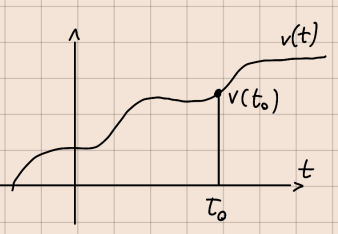
\includegraphics[width=0.5\textwidth]{campionamento.png}
\end{center}

\[
    v(t_0) = \int_{-\infty}^\infty v(t) \delta(t - t_0) dt    
\]

Inolte se v è continua sul dominio 
\[
    V(t) =   \int_{-\infty}^\infty v(t) \delta(t - t) dt \textrm{ moltiplico per } \delta(t - t_0)
\]
\textbf{Dimostrazione}:  
\[
    \begin{split}
        v(t_0) &= v(t) + v(t_0) - v(t)\\
        &v(t_0) \delta(t- t_0) = v(t) \delta(t - t_0) + [v(t_0) - v(t)] \delta(t - t_0)\\
        &\int_{-\infty}^\infty v(t_0) \delta(t - t_0)dt =\\
        &\int_{-\infty}^\infty v(t) \delta(t - t_0) dt +\\
        &+ \underbrace{\int_{-\infty}^\infty \overbrace{\delta(t - t_0)}^{0 \textrm{ per } t \neq t_0} \overbrace{[v(t_0) - v(t)]}^{0 \textrm{ per } t = t_0}}_0dt\\
        &\Rightarrow v(t_0) \underbrace{\int_{-\infty}^\infty \delta(t - t_0) dt}_{1 \textrm{ perché l'impulso è unitario}} = \\
        &= \int_{-\infty}^\infty v(t) \delta(t - t_0) dt\\
        v(t_0) &= \int_{-\infty}^\infty v(t) \delta(t - t_0) dt
    \end{split}    
\] 
\begin{description}
    \item[Osservazione: ] si può scrivere anche come \[v(t_0)  = v(t) \delta (t - t_0)\] 
\end{description}

\section{Segnali a tempo discreto}

\subsection{Impulso unitario discreto o delta di Kroneker}

$\delta: Z \rightarrow R$ è una successione
\[\delta(k) = 
    \begin{cases}
        1, \textrm{ per } k = 0\\
        0, \textrm{ altrimenti}
    \end{cases}  
\]

\begin{SCfigure}[50][h!]
    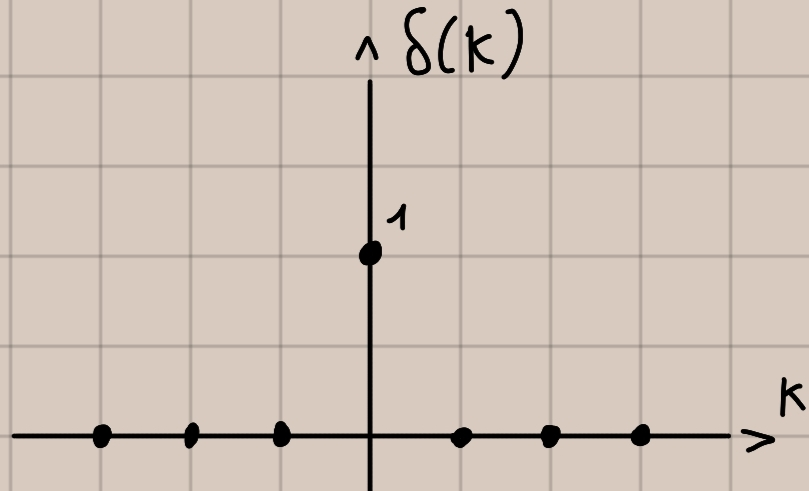
\includegraphics[width=0.5\textwidth]{kroneker.jpg}
    \caption{Delta di Kroneker}
\end{SCfigure}

\subsection{Gradino unitario discreto}

\[
    \delta_{-1}: Z \rightarrow R\qquad \delta_{-1} = \begin{cases}
        1, k \ge 0\\
        0, \textrm{ altrimenti}
    \end{cases}
\]

\begin{SCfigure}[50][h!]
    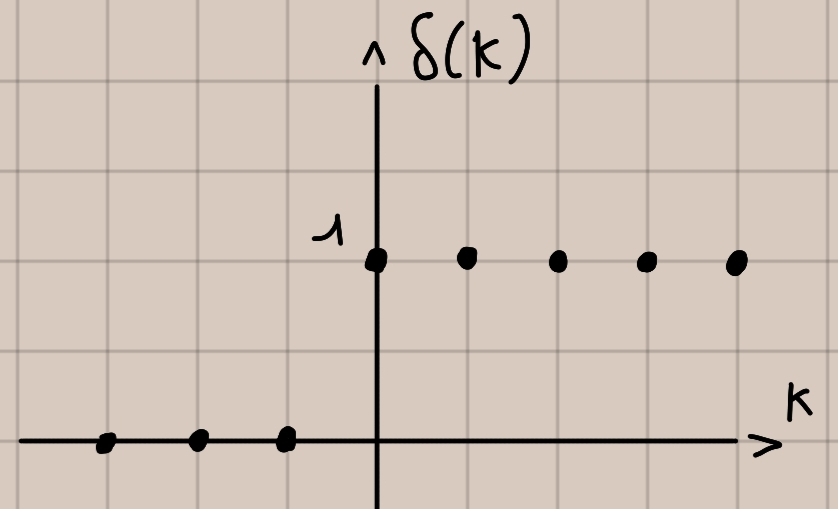
\includegraphics[width=0.5\textwidth]{gradino2.jpg}
    \caption{Gradino}
\end{SCfigure}

\subsection{Rampa discreta unitaria}

\[
    \delta_{-2}: Z \rightarrow R:\qquad \delta_{-2} = \begin{cases}
        k, k \ge 0\\
        0, \textrm{ altrimenti}
    \end{cases}
\]

\begin{SCfigure}[50][h!]
    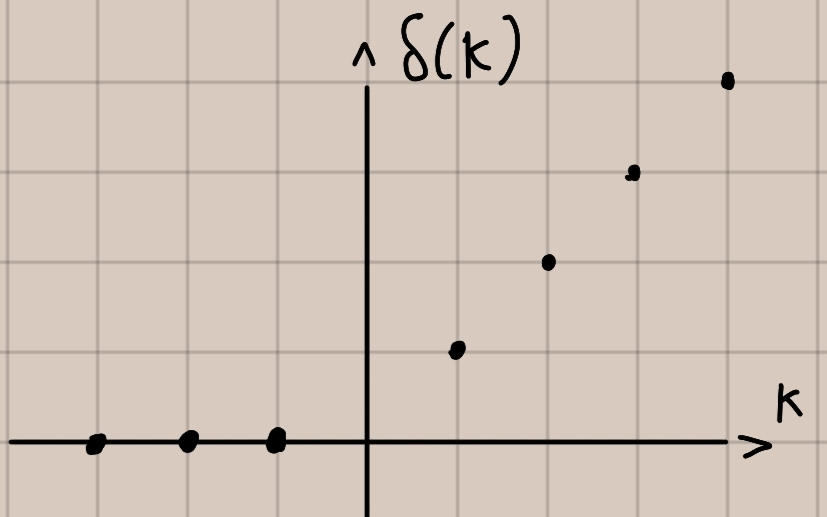
\includegraphics[width=0.5\textwidth]{rampa2.jpg}
    \caption{Rampa}
\end{SCfigure}

\begin{description}
    \item[Osservazione: ] abbiamo che l'integrale dell'impulso del gradino, come serie corrisponde a $\delta_{-1}(k) = \sum_{i = -\infty}^k \delta(i)$ praticamente se io sommo tutti 
    tutti i valori dell'impulso avrò come risultato un qualsiasi valore $k \ge 0$, sommando tutti i valori dell'impulso ottengo il gradino e in modo analogo sommando tutti i valori 
    del gradino fino a k ottendo la rampa $\delta_{-2} = \sum_{i = -\infty}^{k - 1} \delta_{-1} (i)$.
    \item[N.B.: ] la somma nel campo discreto corrisponde all'integrazione nel campo continuo. 
\end{description}

\[
    \delta_{-2} (k) = \sum_{i = -\infty}^{k - 1} \sum_{j = -\infty}^i \delta(ij)
\]

\subsection{Successione esponenziale discreta}

\[
    v : Z \rightarrow R,\quad v(k) = A e^{j\phi} \lambda^k, \textrm{ dove } k \in Z, \phi \in R,\lambda \in C.   
\]
\begin{description}
    \item[Osservazione: ] se scriviamo 
    \[\begin{split}
        \lambda &= \rho(\cos \theta + j\sin \theta)\\
        v(k) &= A r^{j\phi}\rho^k(\cos k \theta + j \sin k \theta) =\\
        &= A e^{j \phi} e^{k \log \phi} e^{jk\theta} = \\
        &= A e^{j\phi} e^{k(\log \phi + j \theta)}
      \end{split}
    \]
\end{description}

\subsection{Successione sinusoidale discreta}
\[
    \begin{split}
    &v: Z \rightarrow R, v(k) = A \cos (\omega k + \phi),\\
    &\textrm{ con } k \in Z, \omega \in R, \phi \in R\\
    &\textrm{ dove } A \textrm{ ampiezza, } \omega \textrm{ pulsazione e } \phi \textrm{ fase.} 
    \end{split}
\]

\begin{description}
    \item[Osservazione: ] $v(k)$ è periodico di periodo $T =  \frac{2\pi}{\omega}$ se e solo se 
    $\omega = 2\pi r$, dove $r \in Q (\omega \textrm{ è un multiplo razionale di } 2\pi)$  
\end{description}

\chapter{Sistema a tempo continuo}

I sistemi possono essere a 
\begin{itemize}
    \item tempo continuo
    \item tempo discreto
\end{itemize}

Un sistema è un modello matematico che formalizza un fenomeno fisico o un processo che in modo deterministico trasforma certi 
input in determinati output. Esempio:
\begin{itemize}
    \item Il pendolo, data una spinta inizierà a muoversi da una parte all'altra, l'input può essere l'impulso della forza applicata
    l'output può essere il movimento nel tempo lungo un asse designato;
    \item Una palla che scivola lungo una collina, l'input può essere simile a quello di prima, l'output sarà il movimento lungo il versante che formerà una specie di mezza parabola;
\end{itemize}

Proprietà:
\begin{enumerate}
    \item Linearità, a una combinazione lineare degli input corrisponde una combinazione lineare degli output 
    \[
        au_1(t) + bu_2(t) \mapsto  av_1(t) + bv_2(t)
    \]
    \item Tempo invarianza, un sistema a tempo continuo è tempo invariante se e solo 
    \[
        u(t) \mapsto v(t) \Rightarrow u(t - \tau) \mapsto v(t - \tau) \forall \tau \in R
    \]
    \item Causalità, un sistema è causale se e solo se l'uscita al momento $\tau$ dipende soltanto dall'ingresso per $t < \tau$ ( $v(\tau)$ dipende soltano
    da $u(t)$ per $t \le \tau$) e non da valori successivi.
\end{enumerate}

\begin{description}
    \item[Osservazione: ] in un sistema causale, l'effetto (output) non può precedere la causa (input) 
    \item[Osservazione: ] considereremo sistemi inizialmente a riposo 
    \[
        (u(t) = 0, t \le \tau \underbrace{\Rightarrow}_{\textrm{sistemi causali}} v(t) = 0, t \le \tau)
    \]  
    Per convenzione $\tau = 0$ (origine del tempo, $t_0$)
    \item[Definizione: ] un sistema a tempo continuo per cui valgono le proprietà di linearità e tempo invarianza si chiama
     sistema LTI (\textbf{Linear time invariant}) 
\end{description}

Proprietà di stabilità asintotica %52:37








\end{document}